\documentclass[10pt]{article}

\usepackage{mathtools, amssymb, bm}
\usepackage{microtype}
\usepackage[utf8]{inputenc}
\usepackage[margin = 0.75in]{geometry}
\usepackage{booktabs}
\usepackage{graphicx}
\usepackage{xcolor}
\usepackage{tikzsymbols}
\usepackage[hidelinks]{hyperref}
\usepackage{titlesec}

\usepackage{wrapfig}

% \titleformat{\section}{\normalsize\bfseries}{\thesection}{1em}{}
\titleformat{\section}{\large\bfseries}{\thesection}{1em}{}
\setcounter{secnumdepth}{0}

\definecolor{colabcol}{HTML}{960018}
\newcommand{\mycolab}[1]{\textcolor{colabcol}{\textsl{Collaborators:}} #1 \\ }
\newcommand{\mycolaba}[1]{\textcolor{colabcol}{\textsl{Collaborators:}} #1}

\title{
    {\Large Homework 3}
}
\author{
    {\normalsize Aiden Kenny}\\
    {\normalsize STAT GR5205: Linear Regression Models}\\
    {\normalsize Columbia University}
}
\date{\normalsize Octover 23, 2020}

\begin{document}

\maketitle

\noindent
Throughout this assingment, we will be using a variety of base R functions to easily obtain the desired measurements. In addition, all measurements
will be rounded to two decimal places or less. 

%' ============================================================================================================================================================
\section{Question 1} \noindent
We are considering the linear regression model 
\begin{align*}
    y = \beta_0 + \beta_1 x + \epsilon,
\end{align*}
where \(\hat{y}\) is the estimated service time for a call, \(x\) is the number of copiers being serviced,
and \(\epsilon \sim \mathrm{N}(0,\sigma^2)\). 
The least-squares estimator model is given by 
\begin{align}
    \hat{y} = -0.58 + 15.04x \label{copier-lm}
\end{align}
% The data and the estimated model are both plotted in Figure \ref{copier-plot}. Visually, it is clear that
% least-squares model fits the data extremely well.
% \begin{figure}[h]
%     \centering
%     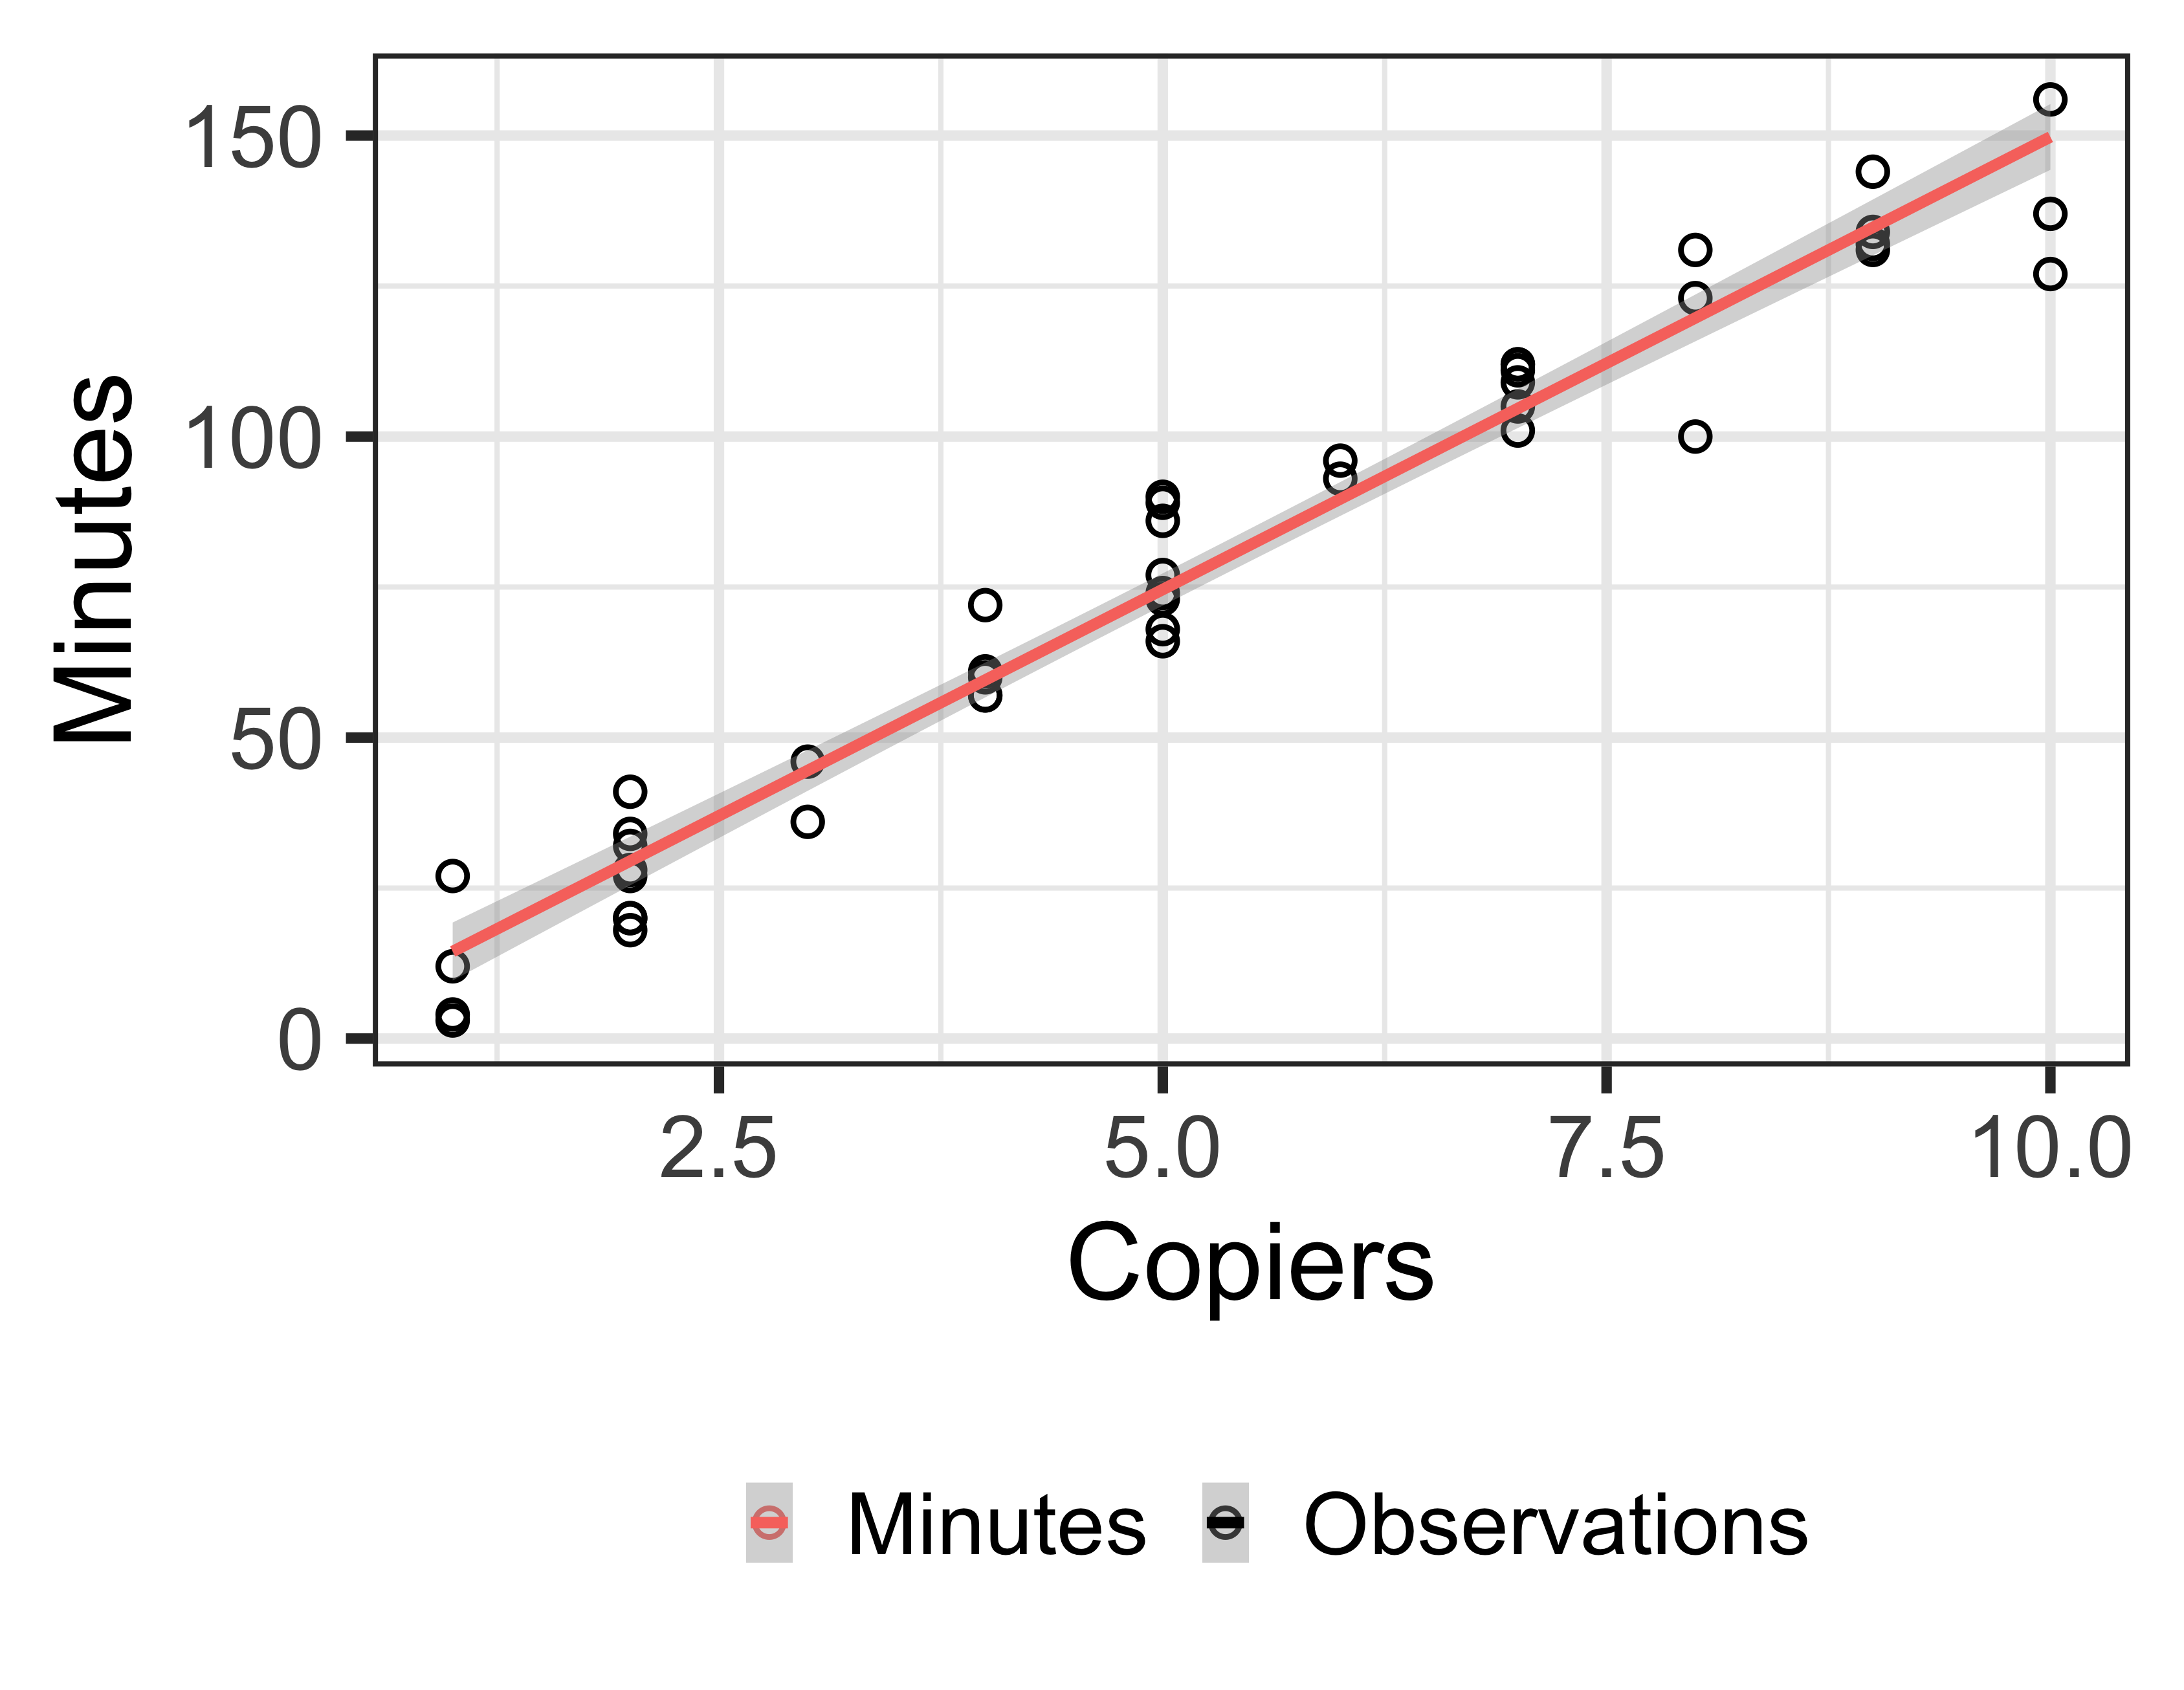
\includegraphics[width = 0.35\textwidth]{img/copier-linear.png}
%     \caption{A plot of model \ref{copier-lm}.}
%     \label{copier-plot}
% \end{figure}
% \begin{wrapfigure}{R}{0.35\textwidth}
%     \centering
%     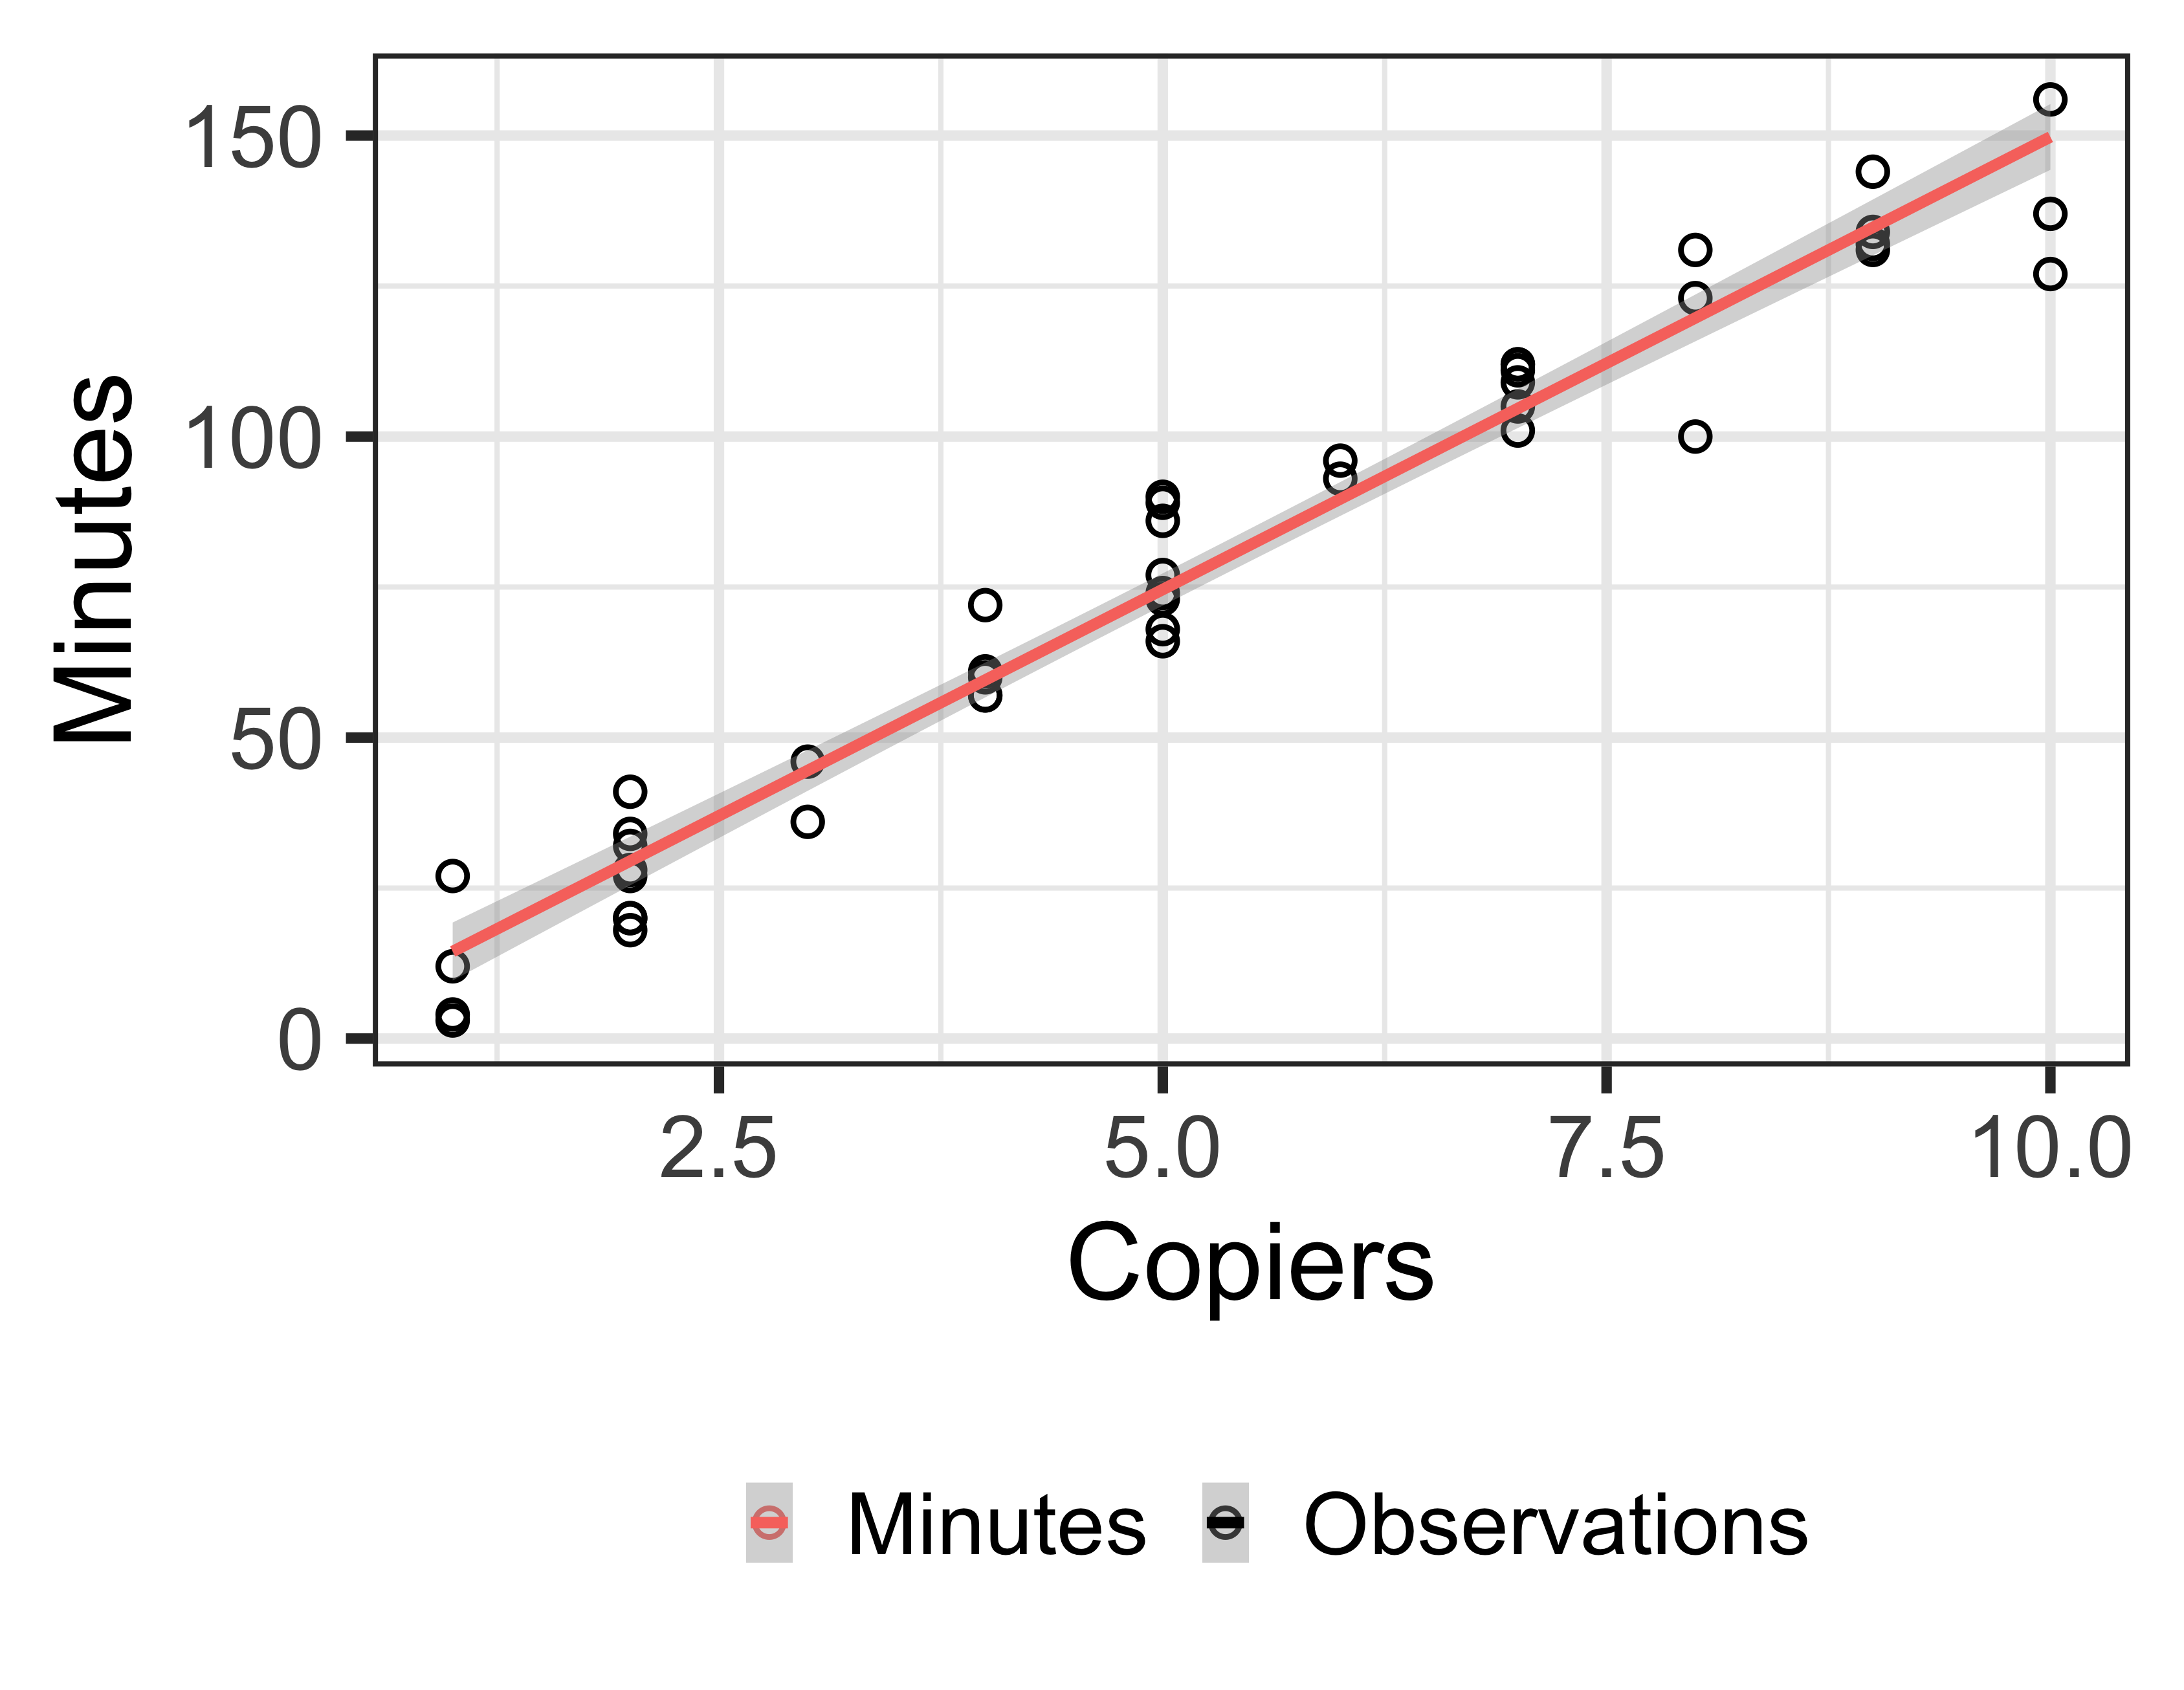
\includegraphics[width = 0.35\textwidth]{img/copier-linear.png}
%     \caption{A plot of model \ref{copier-lm}.}
%     \label{copier-plot}
% \end{wrapfigure}
\begin{itemize}
    \item[(a)] The \(95\%{}\) confidence interval for the mean service time when there are six copiers is given by 
    \begin{align*}
        \mathrm{E}[y] \in \big(86.81, 92.45 \big).
    \end{align*}
    Intuitively, this means that there are six copiers being serviced, we are \(95\%{}\) sure that the average service time for 
    \textsl{all} service times falls within this range. 
    \item[(b)] The \(95\%{}\) prediction interval for the next service time when there are six copiers is 
    \begin{align*}
        \widehat{y} \in \big( 71.44, 107.83 \big).
    \end{align*}
    As expected, we notice that the prediction interval is significantly wider than the confidence interval. 
    \item[(c)] 
    \item[(d)] The ANOVA table has been printed in Table \ref{copier-anova}.
    \begin{table}
        \centering
        \def\arraystretch{1.25}
        \begin{tabular}[ht]{lccccc} \toprule
            Source of Variation & \(\mathrm{df}\) & Sum of Squares & Mean Square & \(f\) & \(\mathrm{Pr}(> f)\) \\\midrule
            Copiers & \(1\) & \(76960\) & \(76960\) & \(968.66\) & \(< 2.2 \times 10^{-16}\) \\
            Residuals & \(43\) & \(3416\) & \(79\) & -- & -- \\
            Total & \(44\) & \(80376\) & -- & -- & -- \\\bottomrule
        \end{tabular}
        \caption{The ANOVA table for model (\ref{copier-lm}).}
        \label{copier-anova}
    \end{table}
    \item[(e)] To determine if there is any linear relationship between \(x\) and \(y\), we conduct an \(F\)-test, where 
    \(H_0 : \beta_1 = 0\) against \(H_a : \beta_1 \neq 0\). From Table \ref{copier-anova}, we see that the associated \(p\)-value is 
    well below the significance level \(\alpha = 0.05\), and so we reject \(H_0\). The data seems to indicate that there is in fact a 
    linear relationship between \(X\) and \(Y\).
    \item[(f)] The total variance explained by the model is known as the \(R^2\) value, and is given by
    \begin{align*}
        R^2 = \frac{\mathrm{SSR}}{\mathrm{SST}} = \frac{76960}{80376} = 0.9575.
    \end{align*}
    That is, about \(95.75\%{}\) of \(Y\)'s variation is explained by model (\ref{copier-lm}), quite a significant reduction. 
\end{itemize}

%' ============================================================================================================================================================
\section{Question 2} \noindent
\begin{itemize}
    \item[(a)] The scatterplot matrix has been printed in Figure \ref{ps-scatterplot}. We can see that there does seem to be a positive correlation between
    all three of the variables. 
    \begin{figure}
        \centering
        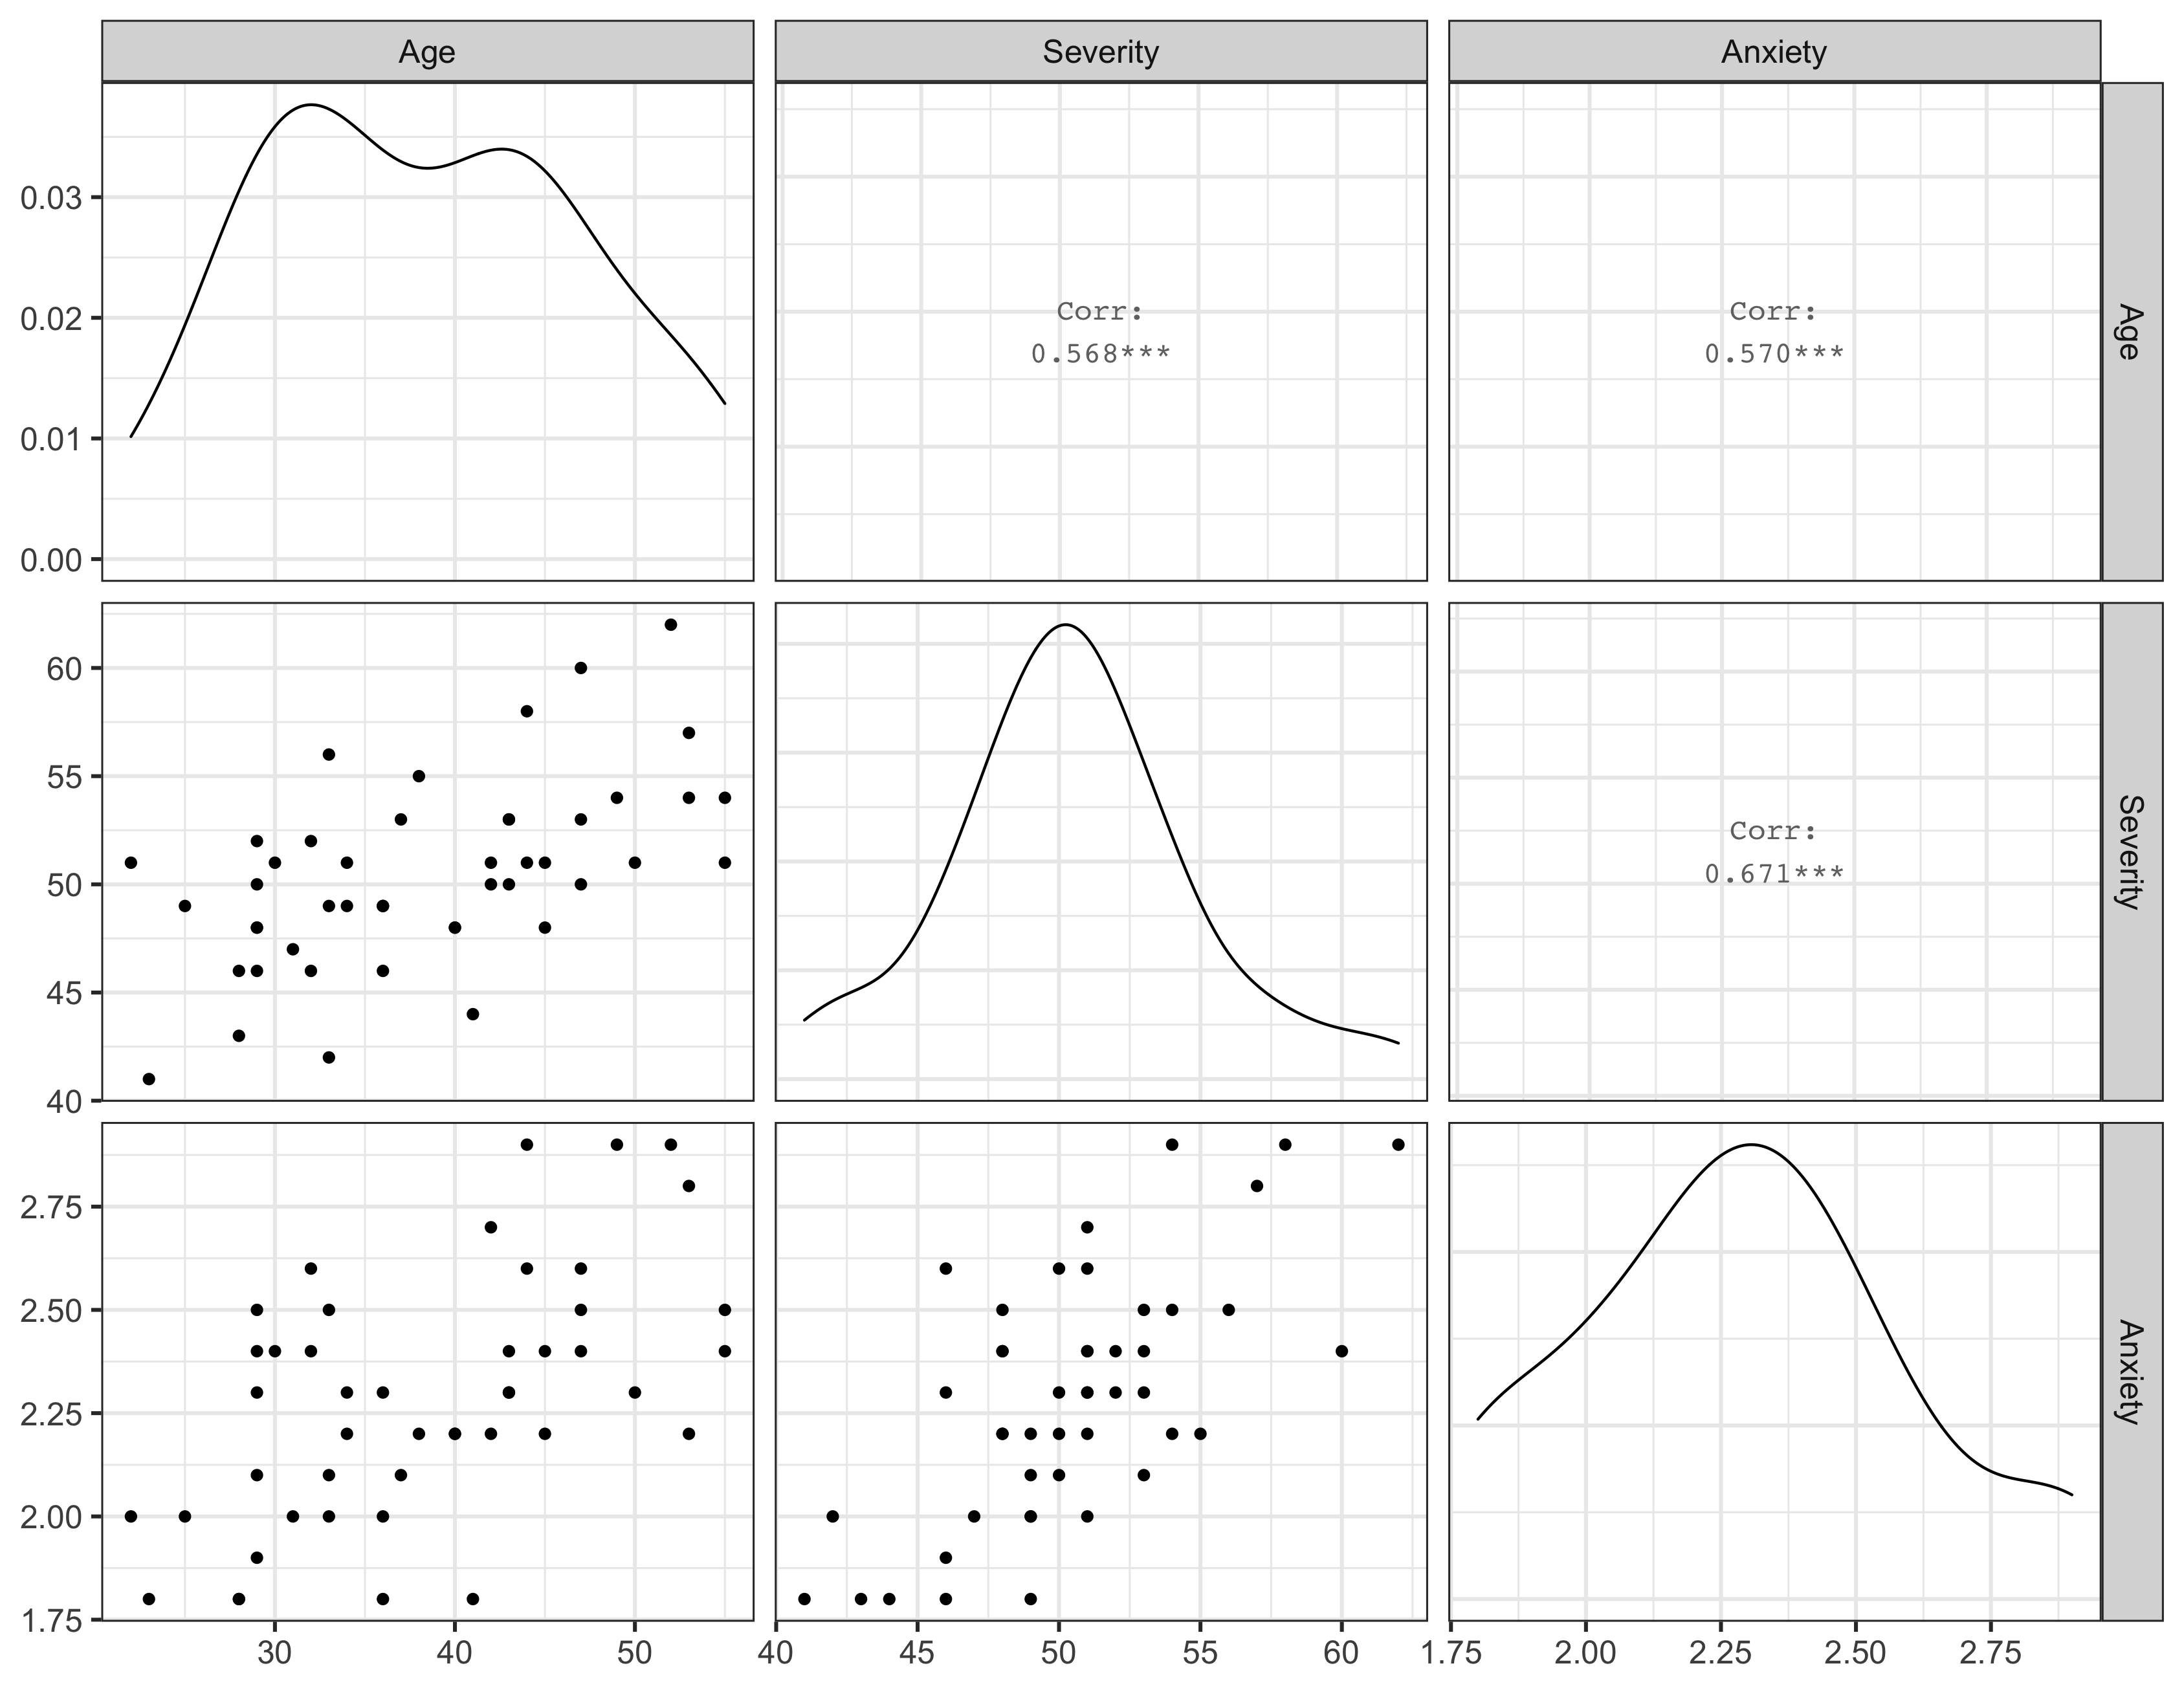
\includegraphics[width = 0.9\textwidth]{img/ps-correlation.png}
        \caption{The scatterplot matrix for {Age}, {Severity}, and {Anxiety}.}
        \label{ps-scatterplot}
    \end{figure}
    \item[(b)] Let \(\mathbf{y}, \mathbf{x}_1, \mathbf{x}_2, \mathbf{x}_3 \in \mathbb{R}^n\) denote {Patient Satisfaction}, {Age},
    {Severity}, and {Anxiety}, respectively, and let 
    \(\mathbf{X} = \begin{bmatrix}
        \mathbf{1} & \mathbf{x}_1 & \mathbf{x}_2 & \mathbf{x}_3
    \end{bmatrix} \in \mathbb{R}^{n \times 4}\).
    The multiple regression model is given by 
    \begin{align}
        \mathbf{y} =  \mathbf{X}\bm{\beta} + \bm{\epsilon},
        \label{ps-lm}
    \end{align}
    where \(\bm{\beta} = (\beta_0, \beta_1, \beta_2, \beta_3)^T\) and \(\bm{\epsilon} \sim \mathrm{N}(\mathbf{0}, \sigma^2 \mathbf{I})\). It is worth 
    emphasizing that \(\bm{\epsilon}\) and \(\mathbf{y}\) are random vectors, while \(\mathbf{X}\) and \(\bm{\beta}\) are fixed. The least-squares estimate
    for \(\bm{\beta}\) is given by 
    \begin{align*}
        \mathbf{b} = \begin{bmatrix}
            b_0 \\ b_1 \\ b_2 \\ b_3
        \end{bmatrix}
        = \begin{bmatrix}
            158.49 \\ -1.14 \\ -0.44 \\ -13.47
        \end{bmatrix},
    \end{align*}
    and our estimated model is given by \(\hat{\mathbf{y}} = \mathbf{X} \mathbf{b}\). What this means is that, when holding all other variables constant, 
    increasing {Severity} by one unit will cause {Satisfaction} to \textsl{decrease} by 0.44.
    \item[(c)] A plot of the residuals against the response and each of the predictors can be found in Figure \ref{ps-residuals}. For each, we see that 
    the residuals appear to be centered around \(0\). We also see that there is no underlying pattern in the residuals as either of the four variables increases. 
    This indicates that none of the model assumptions are violated.
    \begin{figure}
        \centering
        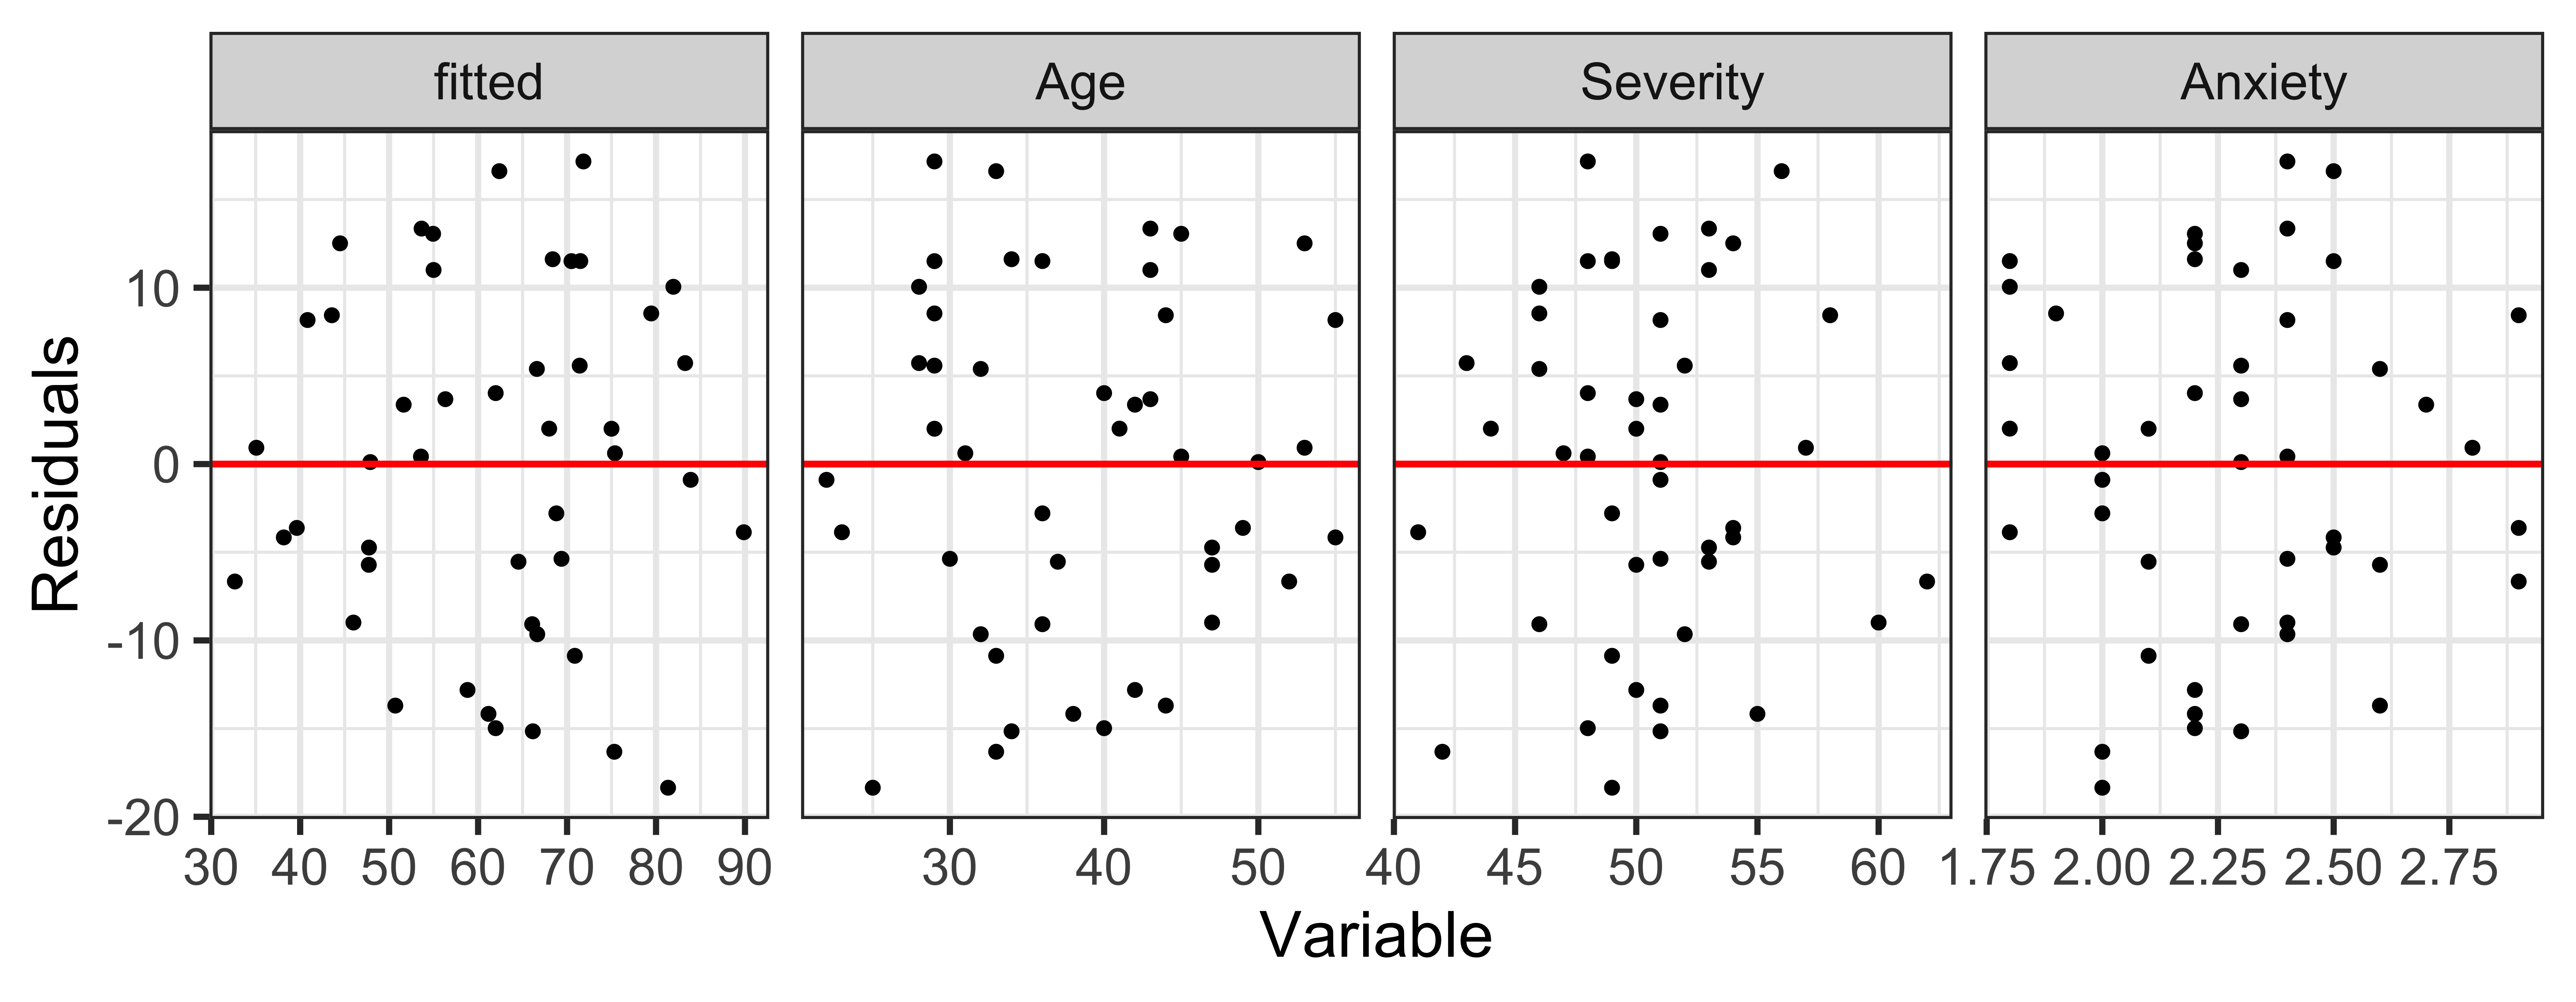
\includegraphics[width = 0.9\textwidth]{img/ps-residuals.png}
        \caption{The residuals plotted against \(\hat{y}\) and each of the predictors.}
        \label{ps-residuals}
    \end{figure}
    \item[(d)] A Q-Q plot of the residuals can be found in Figure \ref{ps-qqplot}. The upper tail of the Q-Q plot greatly deviates from the theoretical values, which could mean that 
    the residuals may not be normally distributed. 
    \begin{figure}
        \centering
        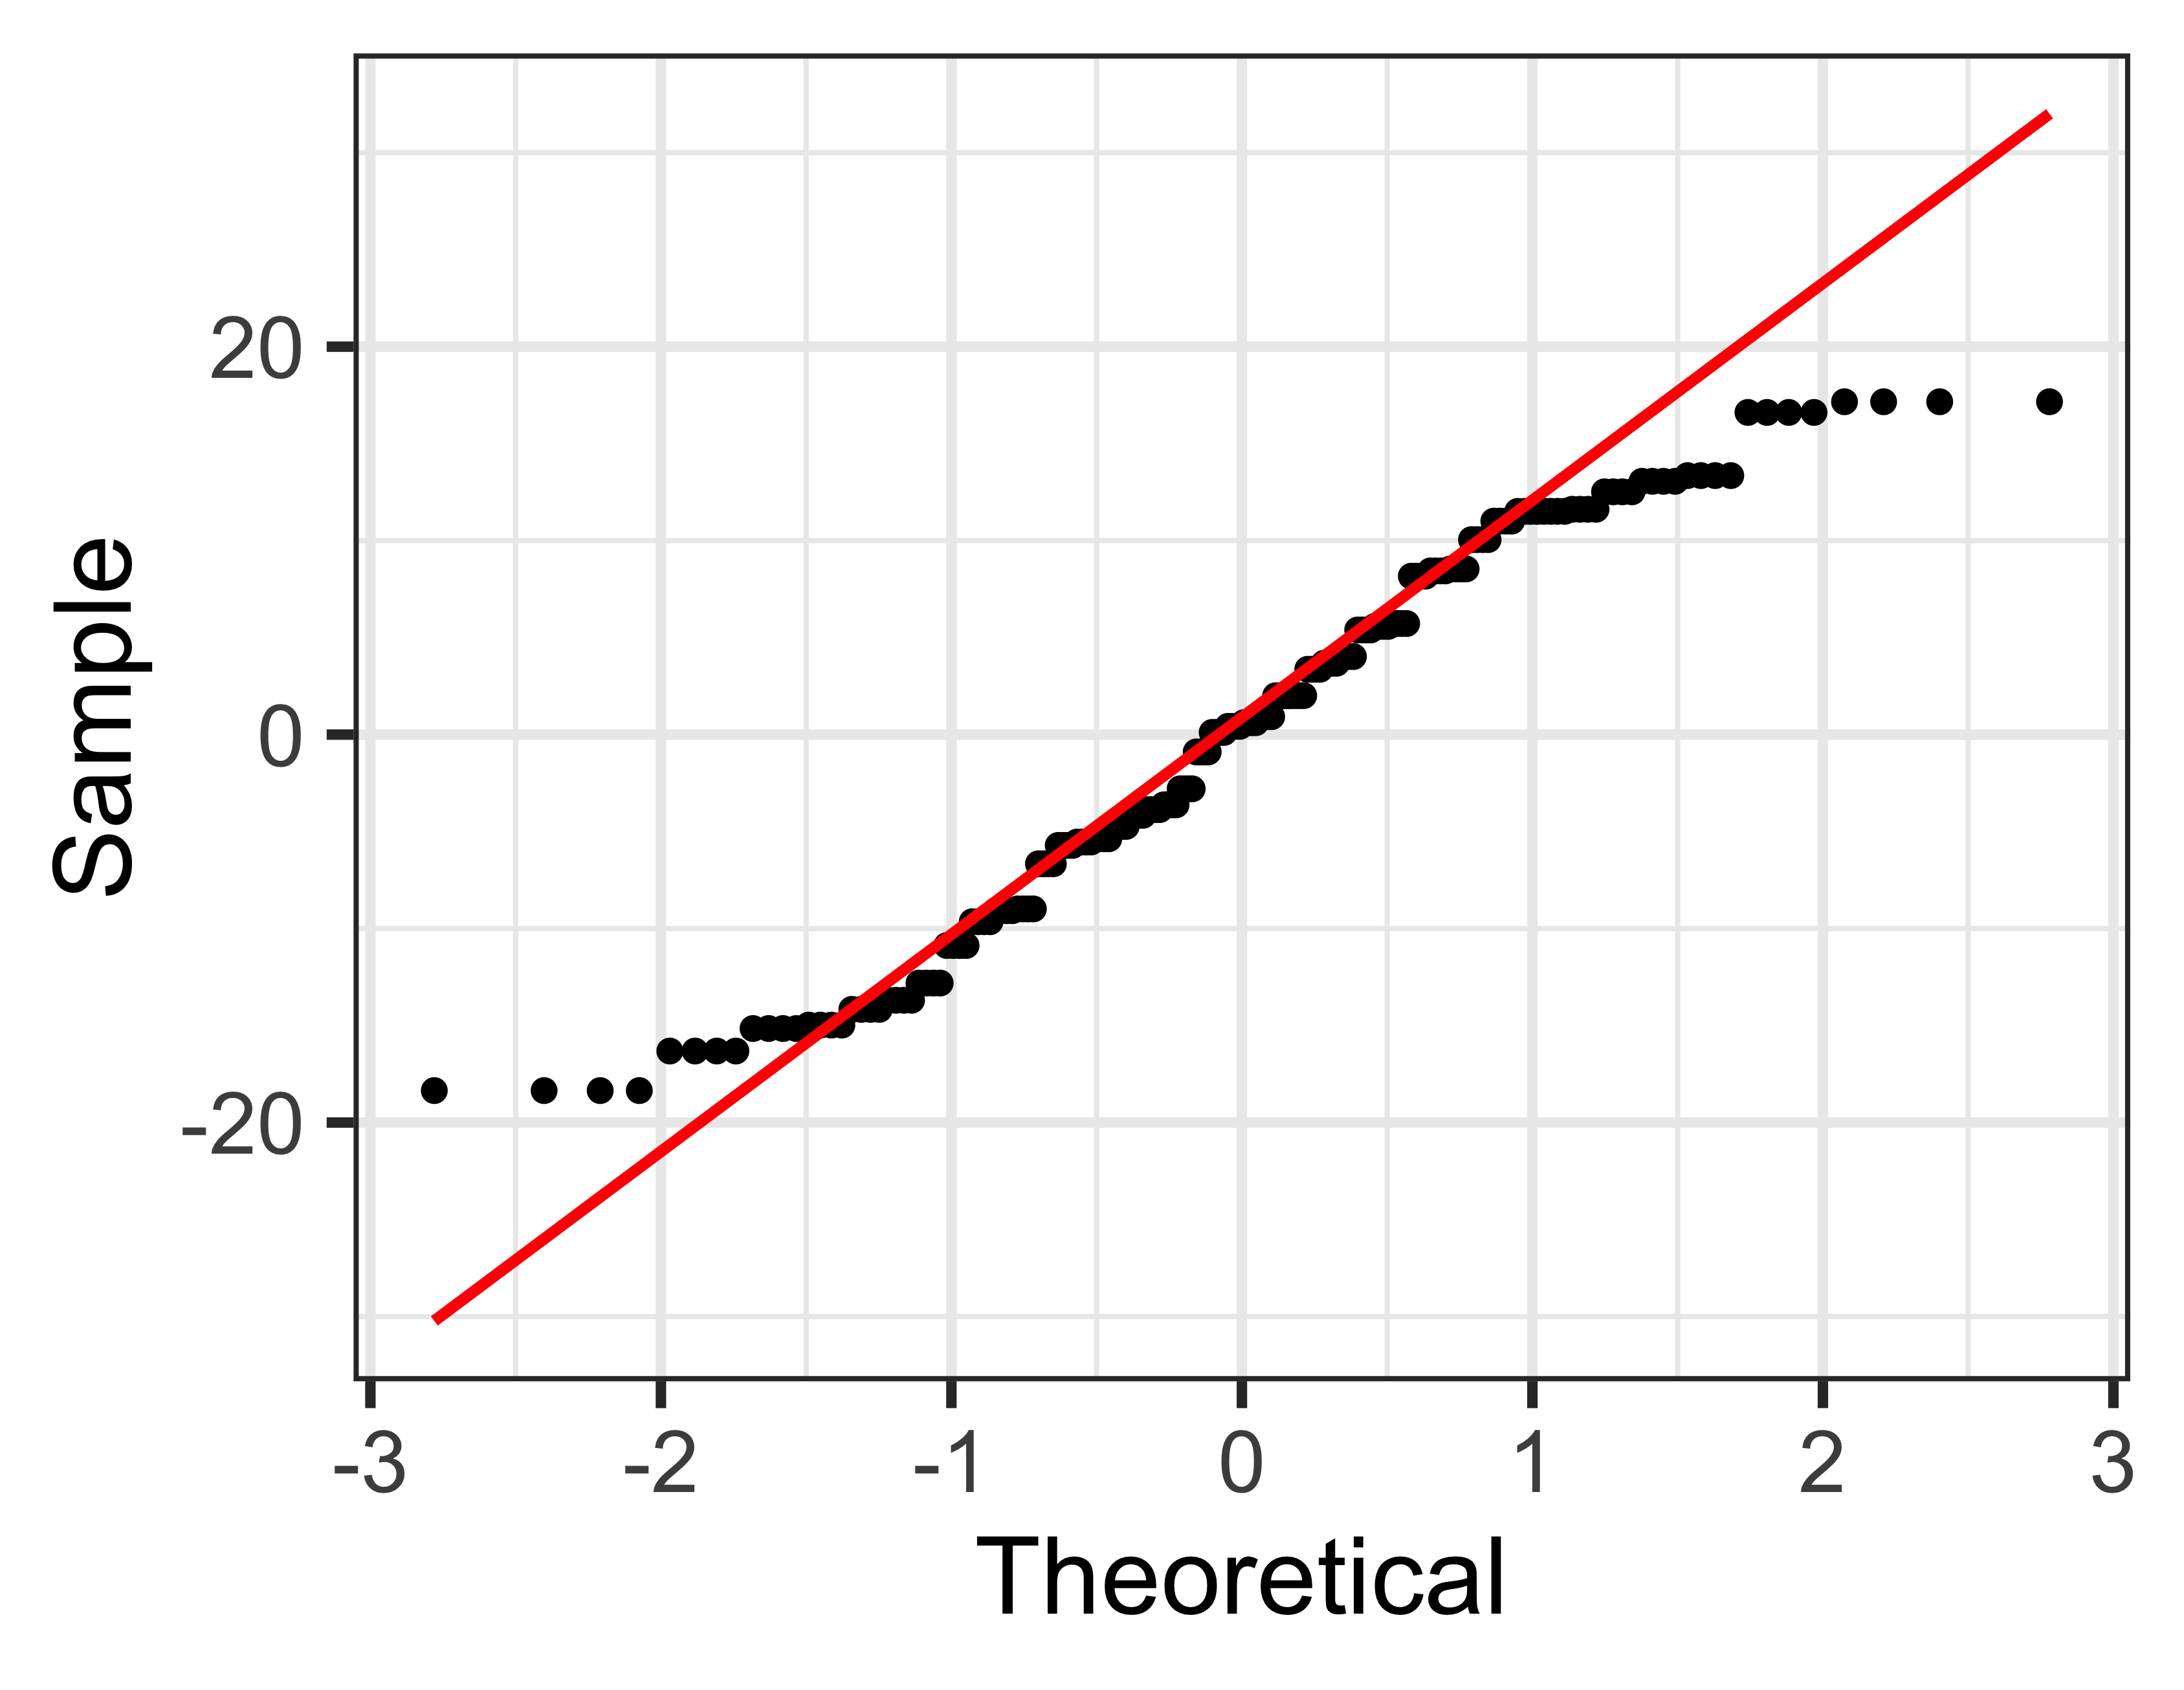
\includegraphics[width = 0.4\textwidth]{img/ps-qqnorm.png}
        \caption{A Q-Q plot of the residuals for model (\ref{ps-lm}).}
        \label{ps-qqplot}
    \end{figure}
\end{itemize}

%' ============================================================================================================================================================
\section{Question 3} \noindent
We are assuming that model (\ref{ps-lm}) is appropriate. 
\begin{itemize}
    \item[(a)] To see if there is \textsl{any} linear relationship between Satisfaction and Age, Severity and Anxiety, we will conduct an \(F\)-test, where 
    \(H_0 : \bm{\beta} = \mathbf{0}\) against \(H_a : \bm{\beta} \neq \mathbf{0}\). Our \(p\)-value is given by 
    \(p \approx 1.542 \times 10^{-10}\), which is significantly lower than \(\alpha = 0.05\). Therefore, we reject \(H_0\); the data indicates that 
    there is a linear relationship. 
    \item[(b)] A joint \(90\%{}\) (not \(95\%{}\)) confidence interval for each of the predictor coefficients is given by 
    \begin{align*}
        \beta_1 &\in \big( -1.50 , -0.78 \big), \\
        \beta_2 &\in \big( -1.27 ,  0.39 \big), \\
        \beta_3 &\in \big( -25.41 , -1.53 \big).
    \end{align*}
    Of the three intervals, we see that the interval for \(\beta_2\) contains zero at this significance level, while the other two intervals do not. That is,
    we are \(90\%{}\) sure that \(\beta_1, \beta_3 \neq 0\) and \(\beta_2 = 0\) (so overall, \(\bm{\beta} \neq \mathbf{0}\)). We believe that 
    Age and Anxiety have a significant effect on Satisfaction, while Severity does not. 
    \item[(c)] The \(R^2\) value here is \(R^2 = 0.6822\), which means about \(68.22\%{}\) of the response's variability is explained by the model, meaning the 
    model is decent. 
    \item[(d)] When a patient is 35 years old, has a severity rating of 45, and an anxiety rating of 2.2, a \(95\%{}\) confidence interval for the average 
    satisfaction rating is \(\big( 63.63, 74.39 \big)\). This means we are \(95\%{}\) sure that for all patients who meet this criteria, the average of 
    all of their satisfaction ratings will fall in this interval. 
    \item[(e)] Given the same conditions, a \(95\%{}\) prediction interval is given by \(\big( 48.012, 90.01 \big)\). We are \(95\%{}\) sure that the satisfaction 
    rating of the next patient we observe will fall in this interval.
\end{itemize}

%' ============================================================================================================================================================
\section{Question 4} \noindent
Let 
\begin{align*}
    \begin{bmatrix}
        X_1 \\ X_2 \\ \epsilon
    \end{bmatrix} \sim \mathrm{N} \left( 
        \begin{bmatrix}
            \mu_1 \\ \mu_2 \\ 0
        \end{bmatrix},
        \begin{bmatrix}
            \sigma^2 & \rho \sigma^2 & 0 \\
            \rho \sigma^2 & \sigma^2 & 0 \\
            0 & 0 & \tilde{\sigma}^2
        \end{bmatrix}
     \right).
\end{align*}
That is, \(X_1 \sim \mathrm{N}(\mu_1, \sigma^2)\), \(X_2 \sim \mathrm{N}(\mu_2, \sigma^2)\) (i.e. \(X_1\) and \(X_2\) have different means but the same 
variance), \(\epsilon \sim \mathrm{N}(0, \tilde{\sigma}^2)\), \(\mathrm{Cor}[X_1, X_2] = \rho\) (which makes \(\rho \sigma^2 = \mathrm{Cov}[X_1, X_2]\)), and 
\(\mathrm{Cov}[X_1, \epsilon] = \mathrm{Cov}[X_2, \epsilon] = 0\). We now consider \(Y = \beta_0 + \beta_1 X_1 + \beta_2 X_2 + \epsilon\), a linear combination. 
\begin{itemize}
    \item[(a)] Since \(Y\) is the sum of normal random variables, \(Y\) must also be normally distributed. It's mean and variance are given by 
    \begin{align*}
        \mathrm{E}[Y]
        &= \mathrm{E}[\beta_0 + \beta_1 X_1 + \beta_2 X_2 + \epsilon]
        = \beta_0 + \beta_1 \mathrm{E}[X_1] + \beta_2 \mathrm{E}[X_2] + \mathrm{E}[\epsilon] \\
        &= \beta_0 + \beta_1 \mu_1 + \beta_2 \mu_2, \\
        \mathrm{Var}[Y]
        &= \mathrm{Var}[\beta_0 + \beta_1 X_1 + \beta_2 X_2 + \epsilon] 
        = \beta_1^2 \mathrm{Var}[X_1] + 2 \beta_1 \beta_2 \mathrm{Cov}[X_1, X_2] + \beta_2^2 \mathrm{Var}[X_2] + \mathrm{Var}[\epsilon] \\
        &= \sigma^2 \big( \beta_1^2 + 2 \rho \beta_1 \beta_2 + \beta_2^2 \big) + \tilde{\sigma}^2.
    \end{align*}
    \item[(b)] We first expand the numerator to get  
    \begin{align*}
        \mathrm{Cov}[X_1, Y]
        &= \mathrm{Cov}[X_1, \beta_0 + \beta_1 X_1 + \beta_2 X_2 + \epsilon]
        = \beta_1 \mathrm{Var}[X_1] + \beta_2 \mathrm{Cov}[X_1, X_2] 
        = \beta_1 \sigma^2 + \rho \beta_2 \sigma^2 \\
        &= \sigma^2 \big( \beta_1 + \rho \beta_2 \big),
    \end{align*}
    and so 
    \begin{align*}
        r_1 
        \coloneqq \frac{\mathrm{Cov}[X_1,Y]}{\sqrt{\mathrm{Var}[X_1] \cdot \mathrm{Var}[Y]}}
        = \frac{\sigma^2 \big( \beta_1 + \rho \beta_2 \big)}{\sqrt{\sigma^2 \Big( \sigma^2 \big( \beta_1^2 + 2 \rho \beta_1 \beta_2 + \beta_2^2 \big) + \tilde{\sigma}^2 \Big)}}
        = \frac{\sigma \big( \beta_1 + \rho \beta_2 \big)}{\sqrt{\sigma^2 \big( \beta_1^2 + 2 \rho \beta_1 \beta_2 + \beta_2^2 \big) + \tilde{\sigma}^2}}.
    \end{align*}
    \item[(c)] We have 
    \begin{align*}
        \mathrm{Cov}[\beta_1 X_1 + \beta_2 X_2, Y]
        &= \beta_1 \mathrm{Cov}[X_1, Y] + \beta_2 \mathrm{Cov}[X_2, Y]
        = \sigma^2 \Big( \beta_1 (\beta_1 + \rho \beta_2) + \beta_2 (\rho \beta_1 + \beta_2) \Big) \\
        &= \sigma^2 \big( \beta_1^2 + 2 \rho \beta_1 \beta_2 + \beta_2^2 \big)
    \end{align*}
    and 
    \begin{align*}
        \mathrm{Var}[\beta_1 X_1 + \beta_2 X_2]
        \beta_1^2 \mathrm{Var}[X_1] + 2 \beta_1 \beta_2 \mathrm{Cov}[X_1, X_2] + \beta_2^2 \mathrm{Var}[X_2]
         = \sigma^2 \big( \beta_1^2 + 2 \rho \beta_1 \beta_2 + \beta_2^2 \big)
    \end{align*}
    (which means \(\mathrm{Cov}[\beta_1 X_1 + \beta_2 X_2, Y] = \mathrm{Var}[\beta_1 X_1 + \beta_2 X_2]\)). Plugging this in gives us 
    \begin{align*}
        r_2 
        &\coloneqq \frac{\mathrm{Cov}[\beta_1 X_1 + \beta_2 X_2, Y]}{\sqrt{\mathrm{Var}[\beta_1 X_1 + \beta_2 X_2] \cdot \mathrm{Var}[Y]}}
        = \frac{\sigma^2 \big( \beta_1^2 + 2 \rho \beta_1 \beta_2 + \beta_2^2 \big)}{\sqrt{\sigma^2 \big( \beta_1^2 + 2 \rho \beta_1 \beta_2 + \beta_2^2 \big) \cdot \Big( \sigma^2 \big( \beta_1^2 + 2 \rho \beta_1 \beta_2 + \beta_2^2 \big) + \tilde{\sigma}^2 \Big)}} \\
        &= \sqrt{\frac{\sigma^2 \big( \beta_1^2 + 2 \rho \beta_1 \beta_2 + \beta_2^2 \big)}{\sigma^2 \big( \beta_1^2 + 2 \rho \beta_1 \beta_2 + \beta_2^2 \big) + \tilde{\sigma}^2}}
    \end{align*}
    \item[(d)] For notational ease, we are going to substitute \(\mathrm{Var}[Y]\) back into \(r_1\) and \(r_2\).
    We first note that 
    \begin{align*}
        r_1^2 = \frac{\sigma^2 (\beta_1 + \rho \beta_2)^2}{\mathrm{Var}[Y]}
        ~~\text{and}~~
        r_2^2 = \frac{\sigma^2 \big( \beta_1^2 + 2 \rho \beta_1 \beta_2 + \beta_2^2 \big)}{\mathrm{Var}[Y]}.
    \end{align*}
    We will start with the assumption \(r_1^2 \le r_2^2\), and then manipulate the inequality until we get a result that will always be true:
    \begin{align}
        & r_1^2 \le r_2^2 \tag{iniital assumption} \\
        & \frac{\sigma^2 (\beta_1 + \rho \beta_2)^2}{\mathrm{Var}[Y]} \le \frac{\sigma^2 \big( \beta_1^2 + 2 \rho \beta_1 \beta_2 + \beta_2^2 \big)}{\mathrm{Var}[Y]} \tag{substituting in} \\
        & \sigma^2 (\beta_1 + \rho \beta_2)^2 \le \sigma^2 \big( \beta_1^2 + 2 \rho \beta_1 \beta_2 + \beta_2^2 \big) \tag{multiply both sides by \(\mathrm{Var}[Y]\)} \\
        & (\beta_1 + \rho \beta_2)^2 \le \beta_1^2 + 2 \rho \beta_1 \beta_2 + \beta_2^2 \tag{divide both sides by \(\sigma^2\)} \\
        & \beta_1^2 + 2 \rho \beta_1 \beta_2 + \rho^2 \beta_2^2 \le \beta_1^2 + 2 \rho \beta_1 \beta_2 + \beta_2^2 \tag{expand left-hand side} \\
        & \rho^2 \beta_2^2 \le \beta_2^2 \tag{subtract \(\beta_1^2 + 2 \rho \beta_1 \beta_2\) from both sides} \\
        & \rho^2 \le 1 \tag{dibide both sides by \(\beta_2^2\)} \\
        & \rho \le 1 \tag{take the square root of both sides}
    \end{align}
    Since \(\rho\) is a correlation, it must be bounded between \(-1\) and \(1\), so the final condition is always true. As a result, we will always
    have \(r_1^2 \le r_2^2\).
\end{itemize}

\end{document}